\section{Externe Schnittstelle}
\label{sec:implementation:externalApi}
Neben der Interaktion mit Benutzern der \textit{TyrolSky}-Anwendung über die \textit{API}-Komponente, wird auch eine Kommunikation mit einem Fremdsystem benötigt. Um Abbuchungen an einem Konto vorzunehmen, wird, wie im Anforderungskatalog unter Abschnitt \ref{sec:Eruierung:sec:Eruierung:technicalRequierements} gefordert, eine externe Anwendung angebunden. Diese Bankenanwendung operiert als eigenständige Anwendung, und simuliert eine Bankenschnittstelle um Kontoabbuchungen von Kunden vorzunehmen. Die Simulationsanwendung selbst ist im nachfolgenden Kapitel \ref{subsec:implementation:bankApi} genauer beschrieben. \\
Der bereits in Abschnitt \ref{subsub:implementation:ChargingCoordinator}  beschriebene Buchungskoordinator verteilt Abbuchungstransaktionen mithilfe von \textit{Sharding} innerhalb des Clusters auf verschiedene Nodes. Jede Transaktion benötigt jedoch eine Kommunikation mit der Bankenschnittstelle, um die Transaktion durchzuführen und sie mit dem Bankensystem abzugleichen.  \\
Dazu wird auf jedem Node welcher Buchungen durchführen kann, das sind alle Nodes mit der Rolle \textit{Domain-Service}, ein \textit{BankingActors} Actor gestartet, welcher für die Kommunikation mit dem Bankenanwendung zuständig ist.
 Möchte nun eine Transaktion eine Kommunikation mit der Bankenanwendung durchführen, so sendet den Befehl zu Kommunikation in Form einer Nachricht an den \textit{BankingActor} welcher sich auf dem gleichen Host befindet wie der Transaktions-Actor. Wird während der Kommunikation zur Bank, der betroffene Transaktions-Actor durch \textit{Sharding} verschoben, betrifft dies nicht den BankingActor selbst, da dieser fix auf jedem Host als eigene Actor Instanz vorhanden ist. 

\subsection{Banken API}
\label{subsec:implementation:bankApi}
Für die Anbindung einer externen Bank wurde eine eigene Software geschrieben, welche einen einfache Banken Schnittstelle zur verfügung stellt. Die \textit{BankChargingAPI} ist komplett getrennt von der restlichen Implementierung der \textit{TyrolSky} Anwendung und wird über eine eigene \textit{REST} Schnittstelle angesprochen. \\
Die Kernaufgabe dieser Bankensimulation ist es, Bankkonnten zu verwalten. Dazu werden in einer relationalen Datenbank Kontoinformationen abgebildet. Dabei hat jedes Konto einen Namen sowie ein aktueller Guthabenstatus. Für die Bankentransaktionen, nicht zu verwechseln mit den Transaktion innerhalb der \textit{TyrolSky}-Anwendung, wird eine eine eigene Tabelle geführt welche Informationen über die Transaktion führt. Jede einkommende Anfrage für eine Kontobewegung wird in einer Transaktion abgebildet. Diese enthält Informationen über den Status der Transaktion sowie deren Transaktionsbetrag. Über die Schnittstelle kann auch der Status einer Transaktion abgefragt werden. Diese Transaktionsstatus Abfrage wird auch von der \textit{TyrolSky}-Anwendung verwendet um die eigene Flugbuchung zu kontrollieren, beschrieben unter Abschnitt \ref{subsub:implementation:ChargingCoordinator}. \\
Für die Implementierung der Simulationsanwendung wurde auf eine \textit{SQL-Datenbank} zurückgegriffen. Jeder Zugriff auf die Datenbank erfolgt in einer Transaktion mit dem strengen Transaktionslevel \textit{Serializable}, wodurch keine Inkonsistenzen der Kontoinformationen entstehen können. Weiters ist durch die Transaktionstabelle eine Nachvollziehbarkeit der Transaktionen möglich. \\
Die Simulationsanwendung \textit{BankChargingAPI} bietet folgende Schnittstellen zur an:
\begin{itemize}
    \litem{ChargeAccount}
        Mit Angabe des gewünschten Kontos sowie des zu abbuchenden Betrages, wird eine Transaktion gestartet. Für den Aufruf, wird weiters eine Transaktionsnummer angegeben, mit welcher später der Status der Transaktion abgefragt werden kann.
    \litem{GetTransactionStatus}
        Durch Angabe der Transaktionsnummer wird der aktuelle Status der Transaktion zurückgegeben. 
\end{itemize}
Durch die Aufteilung in zwei Methoden, ist es möglich im Fehlerfall Transaktionsinformationen nicht zu verlieren. Wird beim Aufruf der \textit{ChargeAccount} Schnittstelle kein Ergebnis zurückgeliefert, so kann der Status trotzdem über \textit{GetTransactionStatus} zu einem späteren Zeitpunkt abgefragt werden.

\section{Testapplikation}
\label{subsec:implementation:TestApplikation} 
Die \textit{TyrolSky}-Anwendung bietet eine Schnittstelle für Enbenutzer an. Um jedoch eine größere Menge an Benutzern, und somit Anfragen zu simulieren wird jedoch eine eigene Testapplikation benötigt. Diese bietet die möglichkeit eine vielzahl an Flügen zu reservieren sowie zu buchen. Weiters wird für jede Anfrage an das \textit{TyrolSky}-System die Anfrage selbst Protokolliert und der Rückgabewert der Anfrage abgespeichert. Dadurch können nach einem Testdurchlauf die Resultate eingesehen und mit dem zustand des getesteten Systems verglichen werden. \\
Die Umsetzung der Testapplikation fordert einen hohen Grad an Parallelisierung, da gleichzeitig eine vielzahl an Anfragen an das System gestellt werden sollen. Aufgrund der Anforderung an eine bestmögliche Parallelisierung, wird die Anwendung mit dem Actor-Model, welches ja für Parallelisierte Anwendungen konzipiert wurde siehe dazu \ref{actor:parallelism}, realisiert. Wie die Implementierung der externen Bankenanwendung, ist auch die Testapplikation eine vollständig eigenständige Anwendung welche, aus sicht der Implementation, keinen Zusammenhang mit der Implementierung der \textit{TyrolSky}-Anwendung besitzt. \\
Jede Anfrage welche zum testenden System durchgeführt wird, wird in einer Datenbanktabelle Protokolliert. Dabei werden Informationen zur Anfrage selbst, wie Flugnummer, Flugdatum und Passagierinformation sowie Informationen zur Buchungs selbst abgespeichert. Der genaue Aufbau der Tabelle \textit{StressTest}, welche alle Informationen über eine Anfrage enthält, ist aus Abbildung \ref{fig:implementation:stressTestDbSchema} zu entnehmen.
\begin{figure}
    \centering
    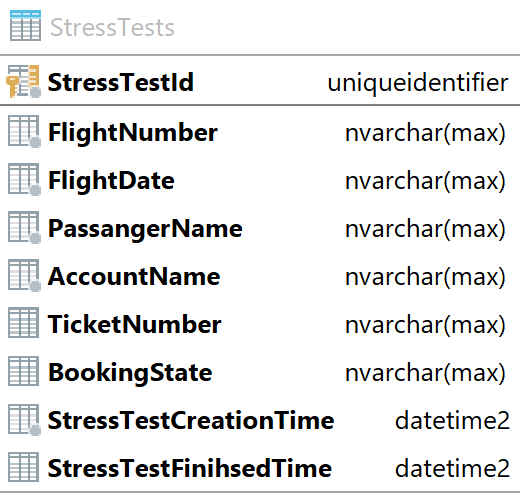
\includegraphics[width=0.4\linewidth]{gfx/implementation/stressTestDbSchema}
    \caption{Das Datenbankschema für die Testapplikation für \textit{TyrolSky}.}
    \label{fig:implementation:stressTestDbSchema}
\end{figure} 

Die Testanwendung wird in Form einer Konsolenanwendung ausgeführt. Dabei kann beim Start der Anwendung über Parameter angegeben werden, welche Flüge in welchem ausmaß gebucht werden sollen. Die Anwendung startet anschließend die entsprechenden Schritte um Flüge zu buchen. 

\subsection{Ablauf eines Testes}
Nach dem Starten der Konsolenanwendung, werden die übergebenen Parameter ausgelesen und das Actor-System gestartet. Anschließend wird die geforderte Anzahl an Buchungen durchgeführt. Dafür wird für jede mögliche Buchung ein eigener Prozess gestartet, welcher in der Tabelle \textit{StressTest} abgebildet wird. Dabei wird zuerst versucht ein Ticket zu reservieren. Konnte eine Reservierung erfolgreicht durchgeführt werden, versucht die Anwendung diese Reservierung zu Buchen. Dafür wird die Kontoinformation, welche für die Buchung verwendet wird, ebenfalls in der Tabelle \textit{StressTest} zum aktuelle getesteten Buchung abgespeichert. Die Testanwendung fragt nach der Buchungsauforderung das zu testenden System nach dem Buchungsresultat, bis dieses einen endgültigen Buchungsstatus zurückliefert. \\
Die einzelnen Buchungsjobs werden dabei nicht alle gleichzeitig gestartet. Alle zwei Sekunden werden 10 neue Jobs gestartet, welche jedoch anschließend parallel bis zur fertigstellung des Jobs weiterlaufen. Die Gesamtanzahl an Jobs wird über die Parameter der Anwendung gesteuert. Ist die Testanwendung beendet, kann das Resultat des Tests in der Datenbank abgefragt werden. Weiters können durch die Angabe der Kontoinformationen die Resultate mit der \textit{BankChargingAPI} Anwendung sowie mit den Entsprchenden Passagierlisten der \textit{TyrolSky} Anwendung verglichen werden.

\subsection{Parameter Beschreibung}
Für die Steuerung und Parametrisierung der \textit{TyrolSky} Testapplikation, können folgende Parameter im zuge des startes der Konsolenanwendung angewandt werden:



